\documentclass[pdf]{beamer}
\mode<presentation>{}

\usepackage[absolute, overlay]{textpos}
\usepackage[style=verbose-ibid,backend=bibtex]{biblatex}
\bibliography{references}

\title{Layer-skipping connections facilitate training of layered networks using equilibrium propagation.}
\author{Jimmy Gammell \and Sae Woo Nam \and Adam N. McCaughan}
\date{July 28, 2020}

\begin{document}

\section{Title} % Total slide count: 7-12 slides
\begin{frame} % title slide
	\titlepage
\end{frame}

\section{Motivation} % 1-2 slides
\begin{frame}
	\frametitle{Motivation: appeal of equilibrium propagation}
	\begin{itemize}
		\item<1-> Equilibrium propagation\autocite{scellier17}: a biologically-motivated learning framework
		\begin{itemize}
			\item<2-> Gradient descent on cost function (alternative to backpropagation)
			\item<3-> Energy-based networks, e.g. continuous Hopfield network
		\end{itemize}
		\item<4-> Advantageous due to simplicity of neurons
		\begin{itemize}
			\item<5-> One computation in both phases of training
			\item<6-> One type of information to transmit in both phases of training
			\item<7-> Biologically plausible (relative to backpropagation)
			\item<8-> Implementable in neuromorphic analog hardware
		\end{itemize}
	\end{itemize}
\end{frame}
\begin{frame}
	\frametitle{Motivation: vanishing gradient problem}
	\begin{itemize}
		\item<1-> Problem: vanishing gradients in layered networks
		\begin{itemize}
			\item<2-> Leads to slow training
			\item<3-> Potential bit-depth issues
			\item<4-> State-of-the-art performance by deep networks
		\end{itemize}
		\item<5-> Not yet solved in simple, biologically-plausible manner
		\item<6-> Original paper: manually tune independent learning rate for each layer
		\item<7-> Per-layer rates unappealing for following reasons:
		\begin{enumerate}
			\item<8-> More hyperparameters to tune
			\item<9-> Inconvenient in neuromorphic hardware
			\item<10-> Seems unlikely in biological systems
		\end{enumerate}
	\end{itemize}
\end{frame}

\section{Introduction} % 1-2 slides
\begin{frame}
	\begin{itemize}
		\frametitle{Introduction}
		\item<1-> Our solution: modified topology including layer-skipping connections
		\item<2-> Addresses above issues with per-layer rates
		\begin{enumerate}
			\item<3-> Two new hyperparameters; constant with depth
			\item<4-> Inspired by small-world topology - observed in biological brains
			\item<5-> Easy to implement in networks with configurable connectivity
		\end{enumerate}
		\item<6-> Improves network training speed
		\item<7-> Increases uniformity with which each layer trains
		\item<8-> Performance similar to that of per-layer rates
	\end{itemize}
\end{frame}

\section{Solution}

\subsection{Original topology illustration}
\begin{frame}
	\frametitle{Original topology}
	\begin{center}
		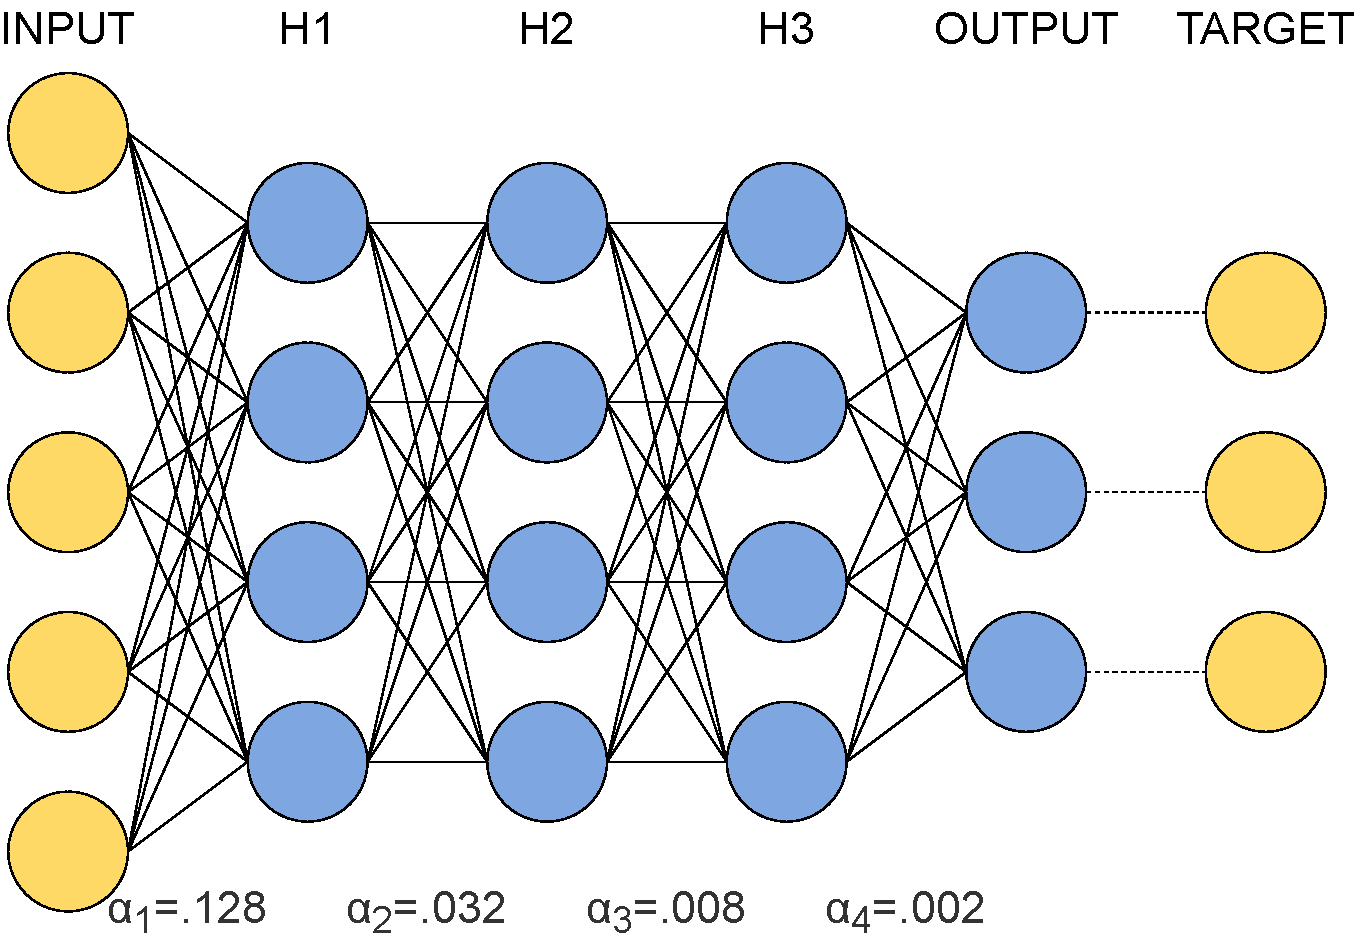
\includegraphics[width=.8\textwidth]{figures/basic_topology_illustration.pdf}
	\end{center}
	\begin{itemize}
		\item From original paper
		\item Per-layer learning rates
	\end{itemize}
\end{frame}

\begin{frame} 
	\frametitle{Our topological modifications}
		\begin{center}
		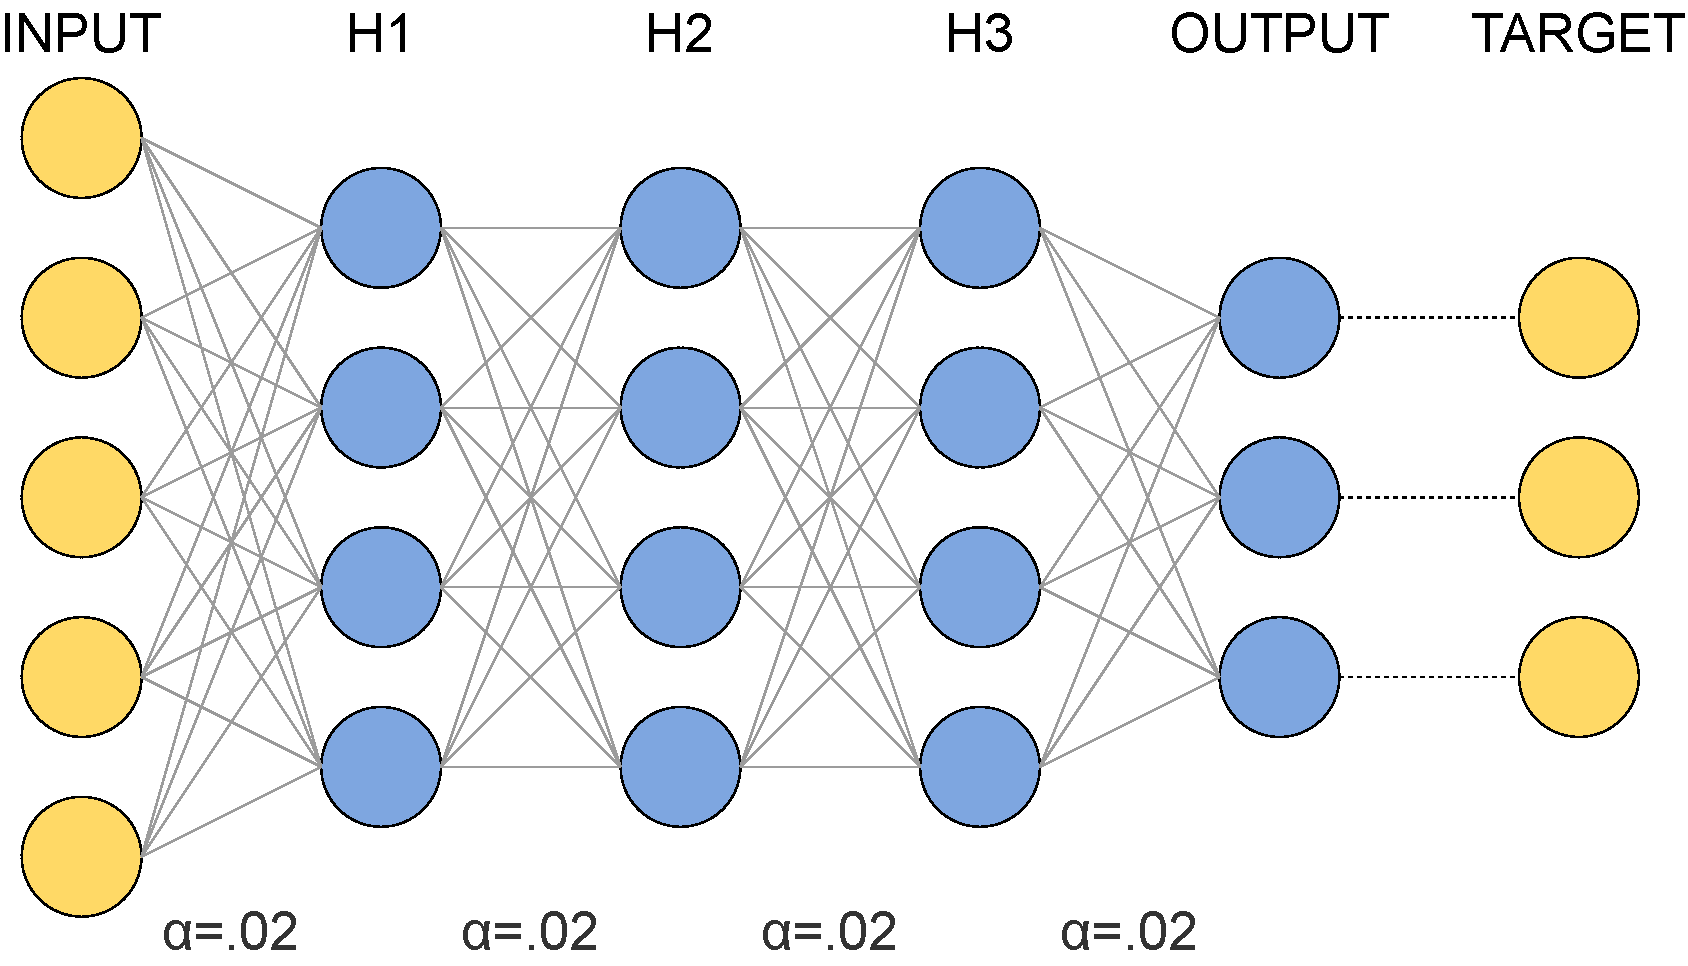
\includegraphics[width=.8\textwidth]{figures/topology_changes_step1.pdf}<1|only@1>
		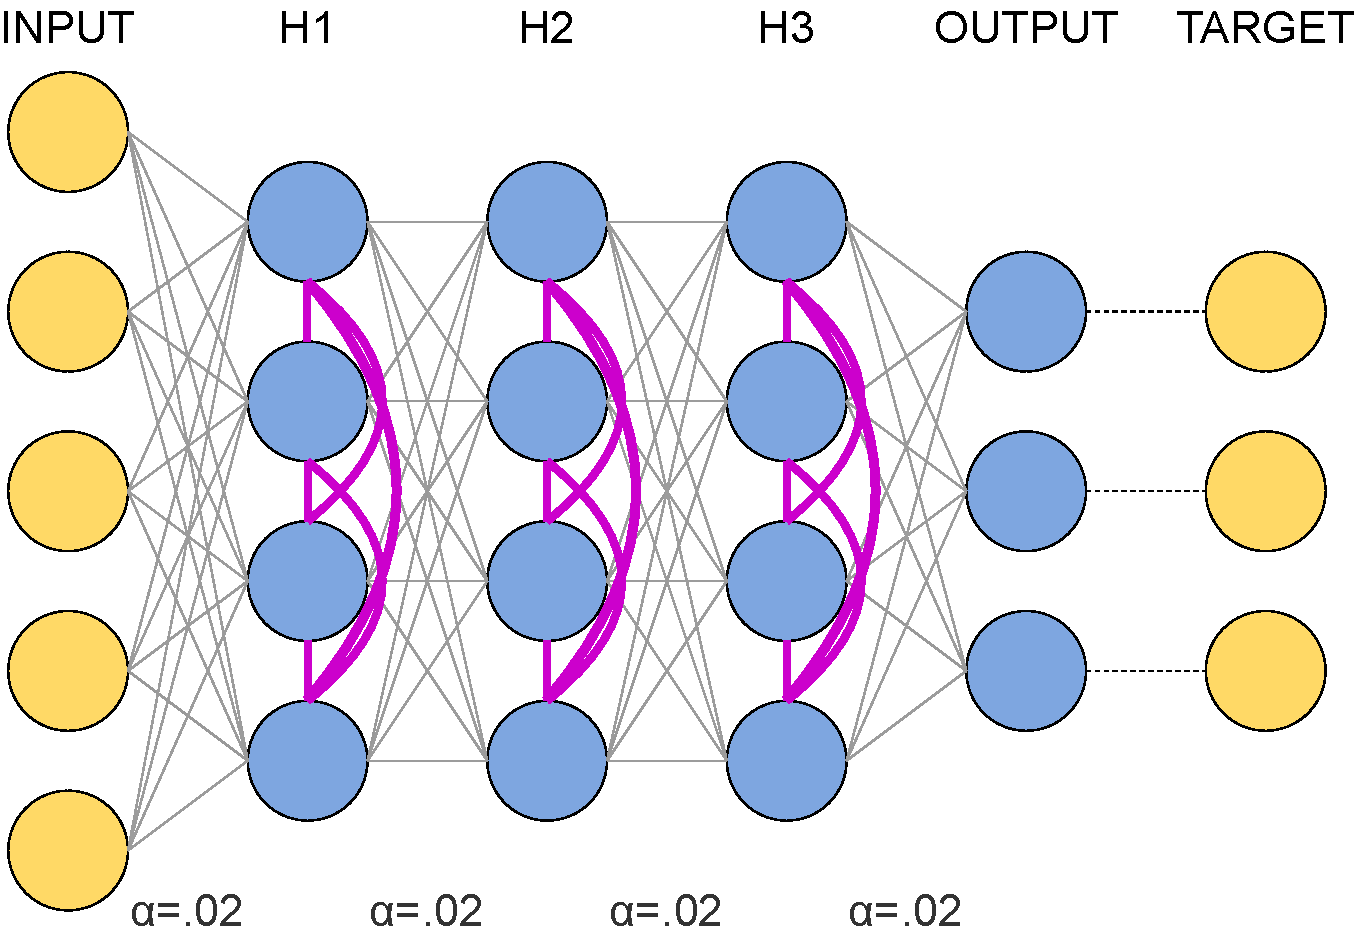
\includegraphics[width=.8\textwidth]{figures/topology_changes_step2.pdf}<2|only@2>
		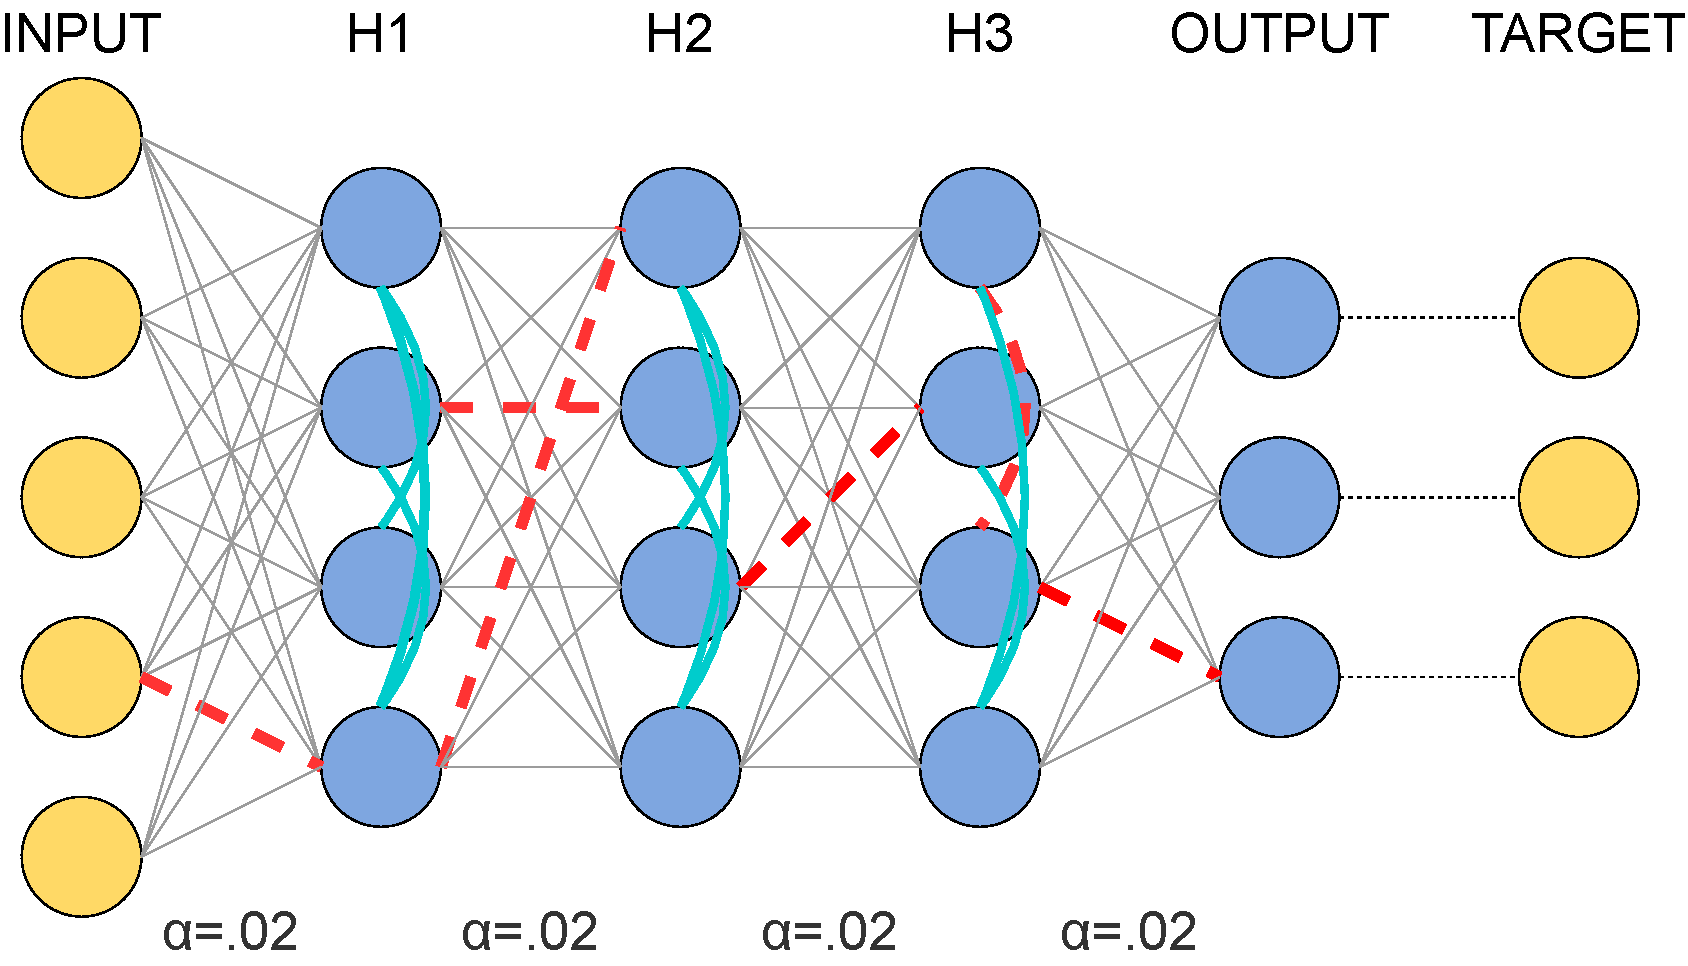
\includegraphics[width=.8\textwidth]{figures/topology_changes_step3.pdf}<3|only@3>
		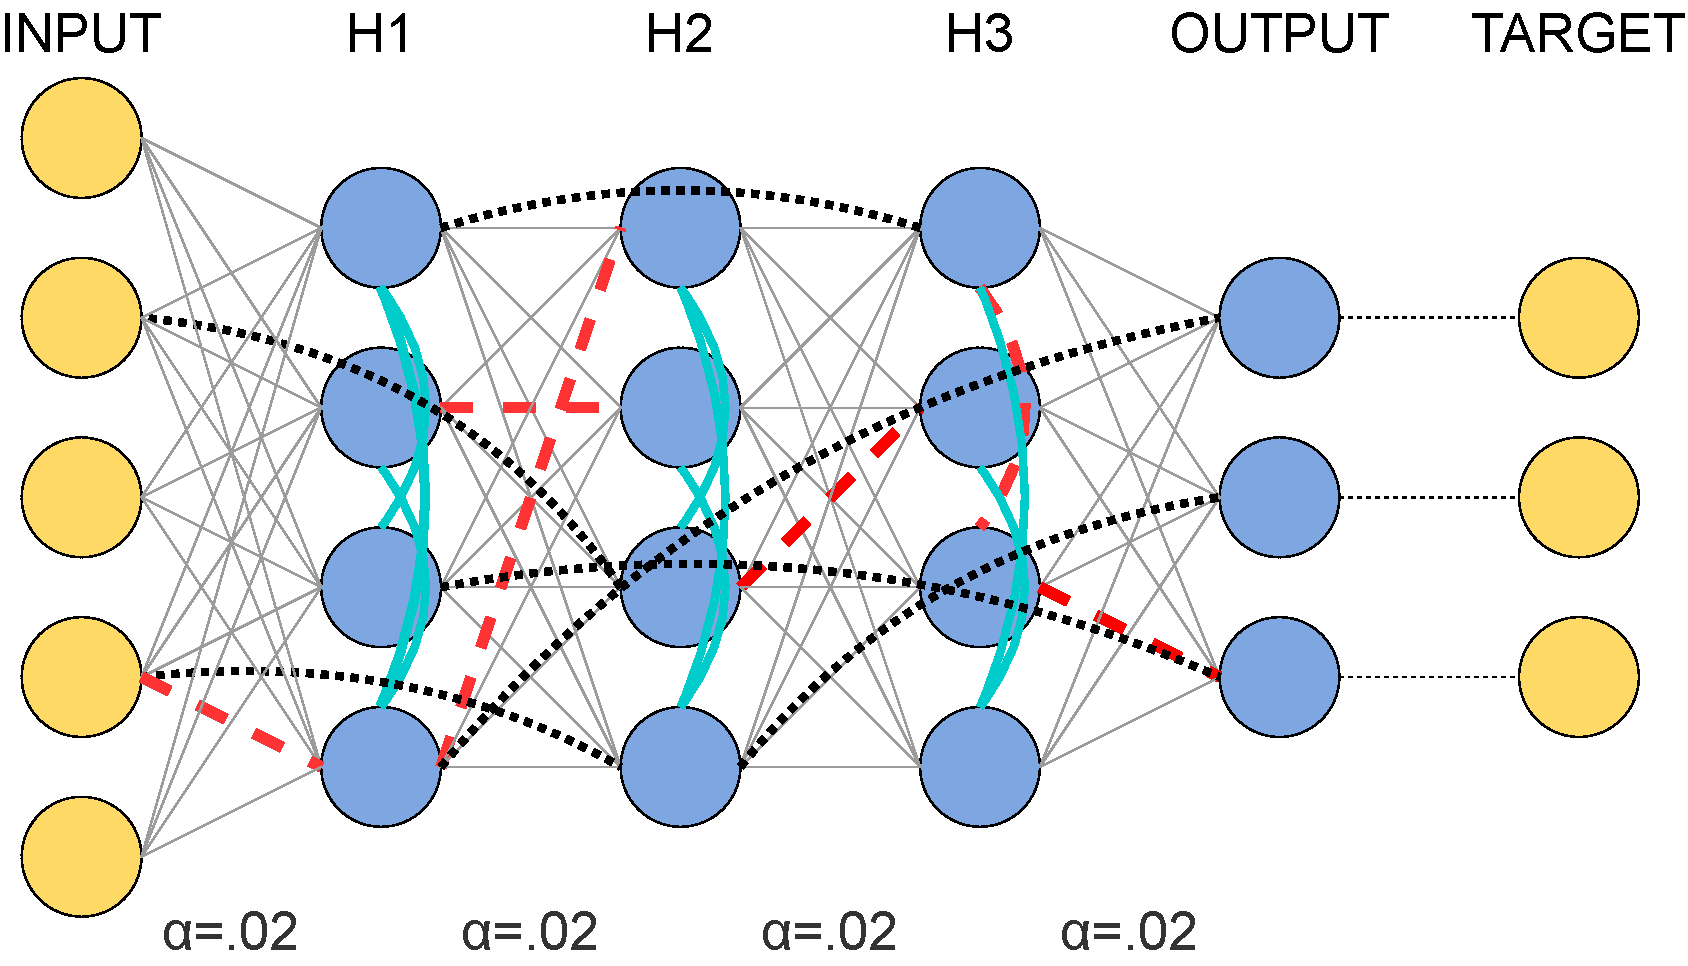
\includegraphics[width=.8\textwidth]{figures/topology_changes_step4.pdf}<4|only@4>
		\end{center}
		\begin{itemize}
			\item<1|only@1> Starting point: original topology
			\item<1|only@1> One learning rate for all layers
		\end{itemize}
		\begin{itemize}
			\item<2|only@2> Hidden layers fully-connected
			\item<2|only@2>[]
		\end{itemize}
		\begin{itemize}
			\item<3|only@3> Consider each connection
			\item<3|only@3> Remove with probability $p$
		\end{itemize}
		\begin{itemize}
			\item<4|only@4> For each removed connection, randomly connect different pair
			\item<4|only@4> No connections in input or output layers
		\end{itemize}
\end{frame}

\section{Results}
\subsection{Performance comparison between topologies}
\begin{frame}
	\frametitle{Results: performance of network with layer-skipping connections}
	\begin{figure}
		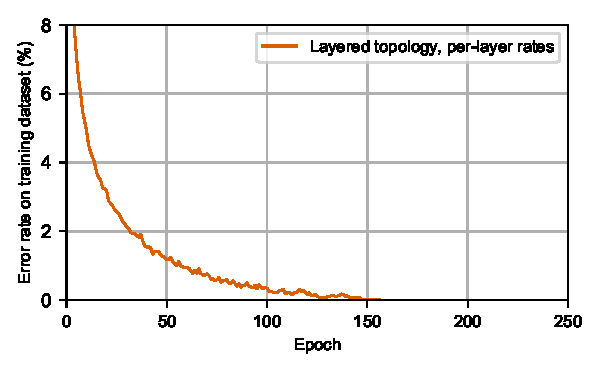
\includegraphics[width=\textwidth]{figures/performance_original.pdf}
	\end{figure}
\end{frame}
\begin{frame}
	\frametitle{Results: performance of network with layer-skipping connections}
	\begin{figure}
		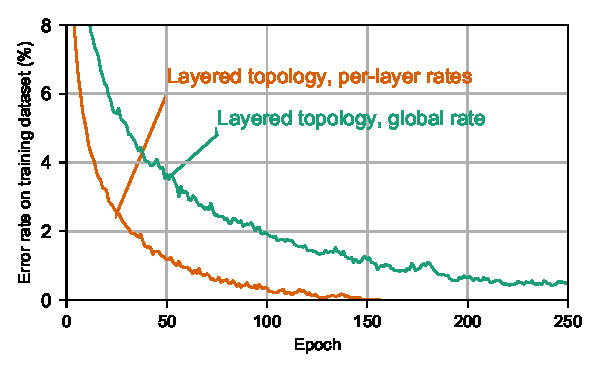
\includegraphics[width=\textwidth]{figures/performance_original+global.pdf}
	\end{figure}
\end{frame}
\begin{frame}
	\frametitle{Results: performance of network with layer-skipping connections}
	\begin{figure}
		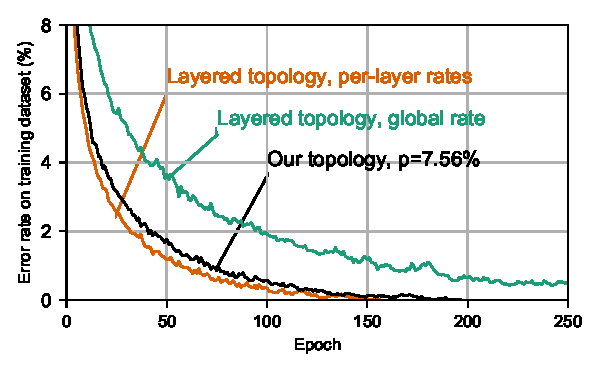
\includegraphics[width=\textwidth]{figures/performance_original+global+ours.pdf}
	\end{figure}
\end{frame}
\subsection{Layer training rate comparison between topologies}
\begin{frame}
	\frametitle{Results: effect on training rates of layers}
	\begin{figure}
		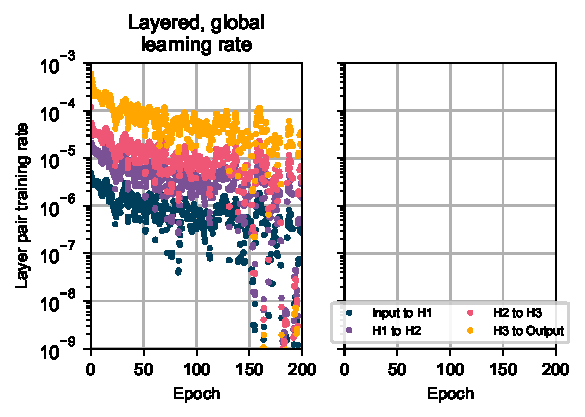
\includegraphics[width=\textwidth]{figures/perlayer_global.pdf}
	\end{figure}
\end{frame}
\begin{frame}
	\frametitle{Results: effect on training rates of layers}
	\begin{figure}
		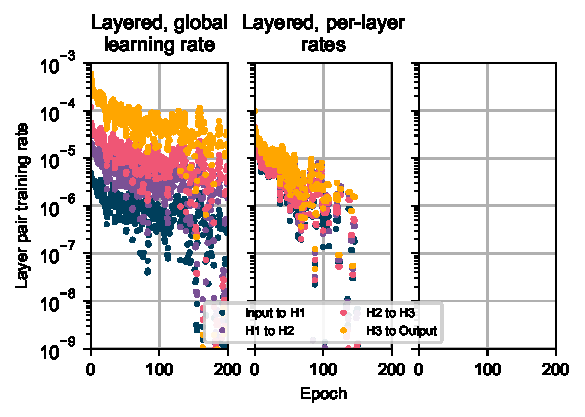
\includegraphics[width=\textwidth]{figures/perlayer_global+original.pdf}
	\end{figure}
\end{frame}
\begin{frame}
	\frametitle{Results: effect on training rates of layers}
	\begin{figure}
		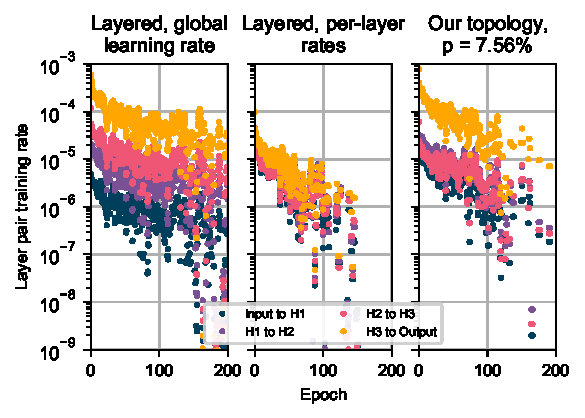
\includegraphics[width=\textwidth]{figures/perlayer_global+original+ours.pdf}
	\end{figure}
\end{frame}

\begin{frame}
	\frametitle{Results: takeaways}
	\begin{itemize}
		\item<1-> Our topology increases training speed
		\begin{itemize}
			\item<2-> Much faster than original topology, one learning rate
			\item<3-> Slightly slower than per-layer rates
		\end{itemize}
		\item<4-> Layers train in more-uniform manner
		\begin{itemize}
			\item<5-> Output layer faster - no added connections to target layer
		\end{itemize}
		\item<6-> Good solution where simplicity, biological plausibility are important
			
	\end{itemize}
\end{frame}

\section{Directions for future research}
\begin{frame}
	\frametitle{Directions for future research}
	\begin{itemize}
		\item<1-> Try on harder datasets (e.g. CIFAR, ImageNet) where depth is very important
		\item<2-> Effect of $p$ on test error
		\item<3-> Effectiveness on deeper networks
		\item<4-> Try training a network with added layer-skipping connections, then removing them afterwards
	\end{itemize}
\end{frame}

\end{document}